%%%%%%%%%%%%%%%%%%%%%%%%%%%%%%%%%%%%%%%%%%%%%%%%%%%%%%%%%%
% # Appendix: Variance Results
%%%%%%%%%%%%%%%%%%%%%%%%%%%%%%%%%%%%%%%%%%%%%%%%%%%%%%%%%%

\chapter{Variance Results}\label{app-results-variance}

%========================================================%
\section{SPRT variance data}\label{app-var-spr}
%========================================================%

% ORC Means
% \DTLloaddb{dt-spr-var}{../analysis/tables/spr_accuracy_var.csv}
% \ExplSyntaxOn
% \tl_clear:N \tblrbody
% \tl_build_begin:N \tblrbody
% \DTLforeach[\equal{\study}{ORC}]{dt-spr-var}{\study=study,\coli=Group,\colii=Dependency,\coliii=Environment,\coliv=Mean,\colv=$CI$}{\tl_build_put_right:Ne \tblrbody {\exp_not:V \coli & \exp_not:V \colii & \exp_not:V \coliii & \exp_not:V \coliv & \exp_not:V \colv\\}}
% \tl_build_end:N \tblrbody
% \ExplSyntaxOff
% \begin{longtblr}[caption={Variance for comprehension-question accuracy in the ORC self-paced reading task}, label={tblr:app-orc-spr-var}, expand=\tblrbody]{colspec={XXXX[r]X[r]}}\toprule
% Group & Dependency & Environment & Mean & 95\% \textit{CI}\\\midrule
% \tblrbody\bottomrule
% \end{longtblr}
% \vspace{-12pt}

% SRC Means
% \ExplSyntaxOn
% \tl_clear:N \tblrbody
% \tl_build_begin:N \tblrbody
% \DTLforeach[\equal{\study}{SRC}]{dt-spr-var}{\study=study,\coli=Group,\colii=Dependency,\coliii=Environment,\coliv=Mean,\colv=$CI$}{\tl_build_put_right:Ne \tblrbody {\exp_not:V \coli & \exp_not:V \colii & \exp_not:V \coliii & \exp_not:V \coliv & \exp_not:V \colv\\}}
% \tl_build_end:N \tblrbody
% \ExplSyntaxOff
% \begin{longtblr}[caption={Variance for comprehension-question accuracy in the SRC self-paced reading task}, label={tblr:app-src-spr-var}, expand=\tblrbody]{colspec={XXXX[r]X[r]}}\toprule
% Group & Dependency & Environment & Mean & 95\% \textit{CI}\\\midrule
% \tblrbody\bottomrule
% \end{longtblr}
% \vspace{-12pt}

% ORC Figure
% \begin{figure}
% \caption{Mean variance for comprehension-question accuracy in the ORC self-paced reading task} \label{fig:app-orc-spr-var}
% \raggedright\setstretch{1}
% 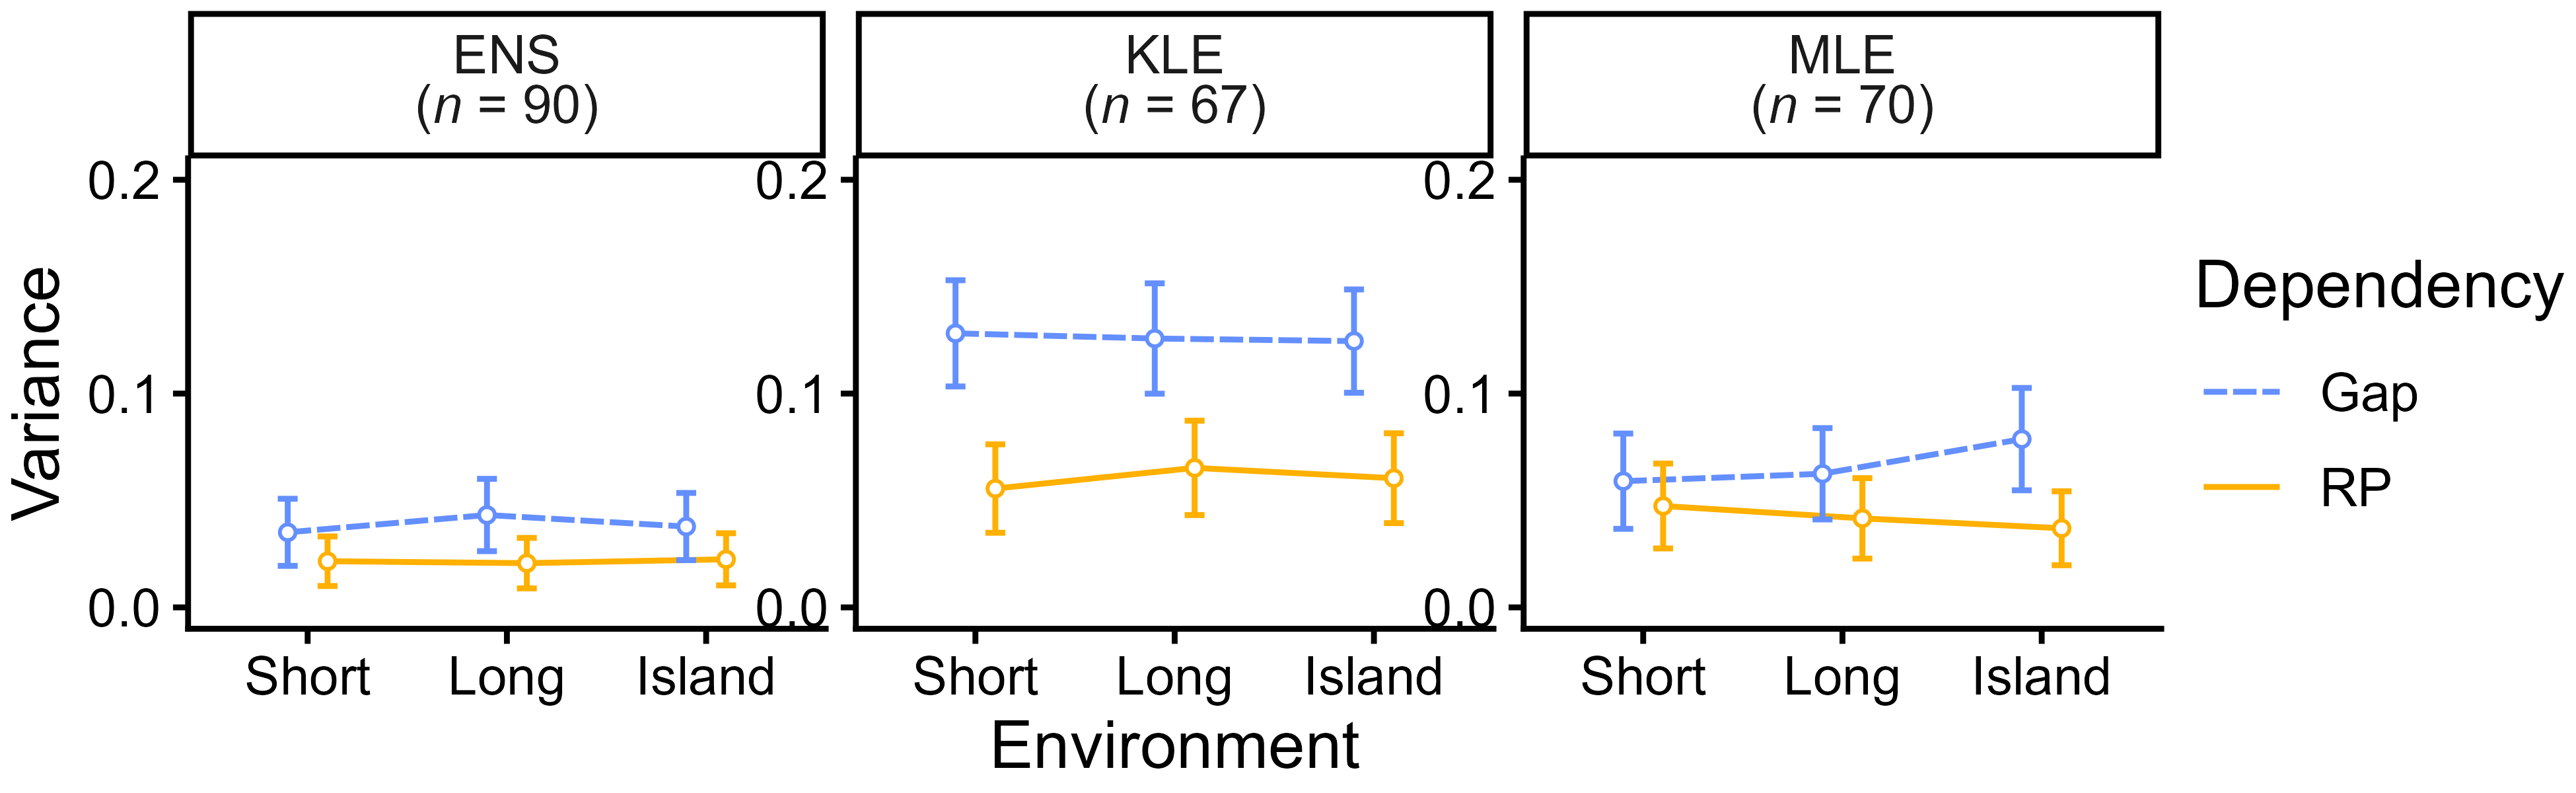
\includegraphics{../analysis/plots/orc_spr_accuracy_var.png}
% \vspace{-12pt}
% \end{figure}

% SRC Figure
% \begin{figure}
% \caption{Mean variance for comprehension-question accuracy in the SRC self-paced reading task} \label{fig:app-src-spr-var}
% \raggedright\setstretch{1}
% 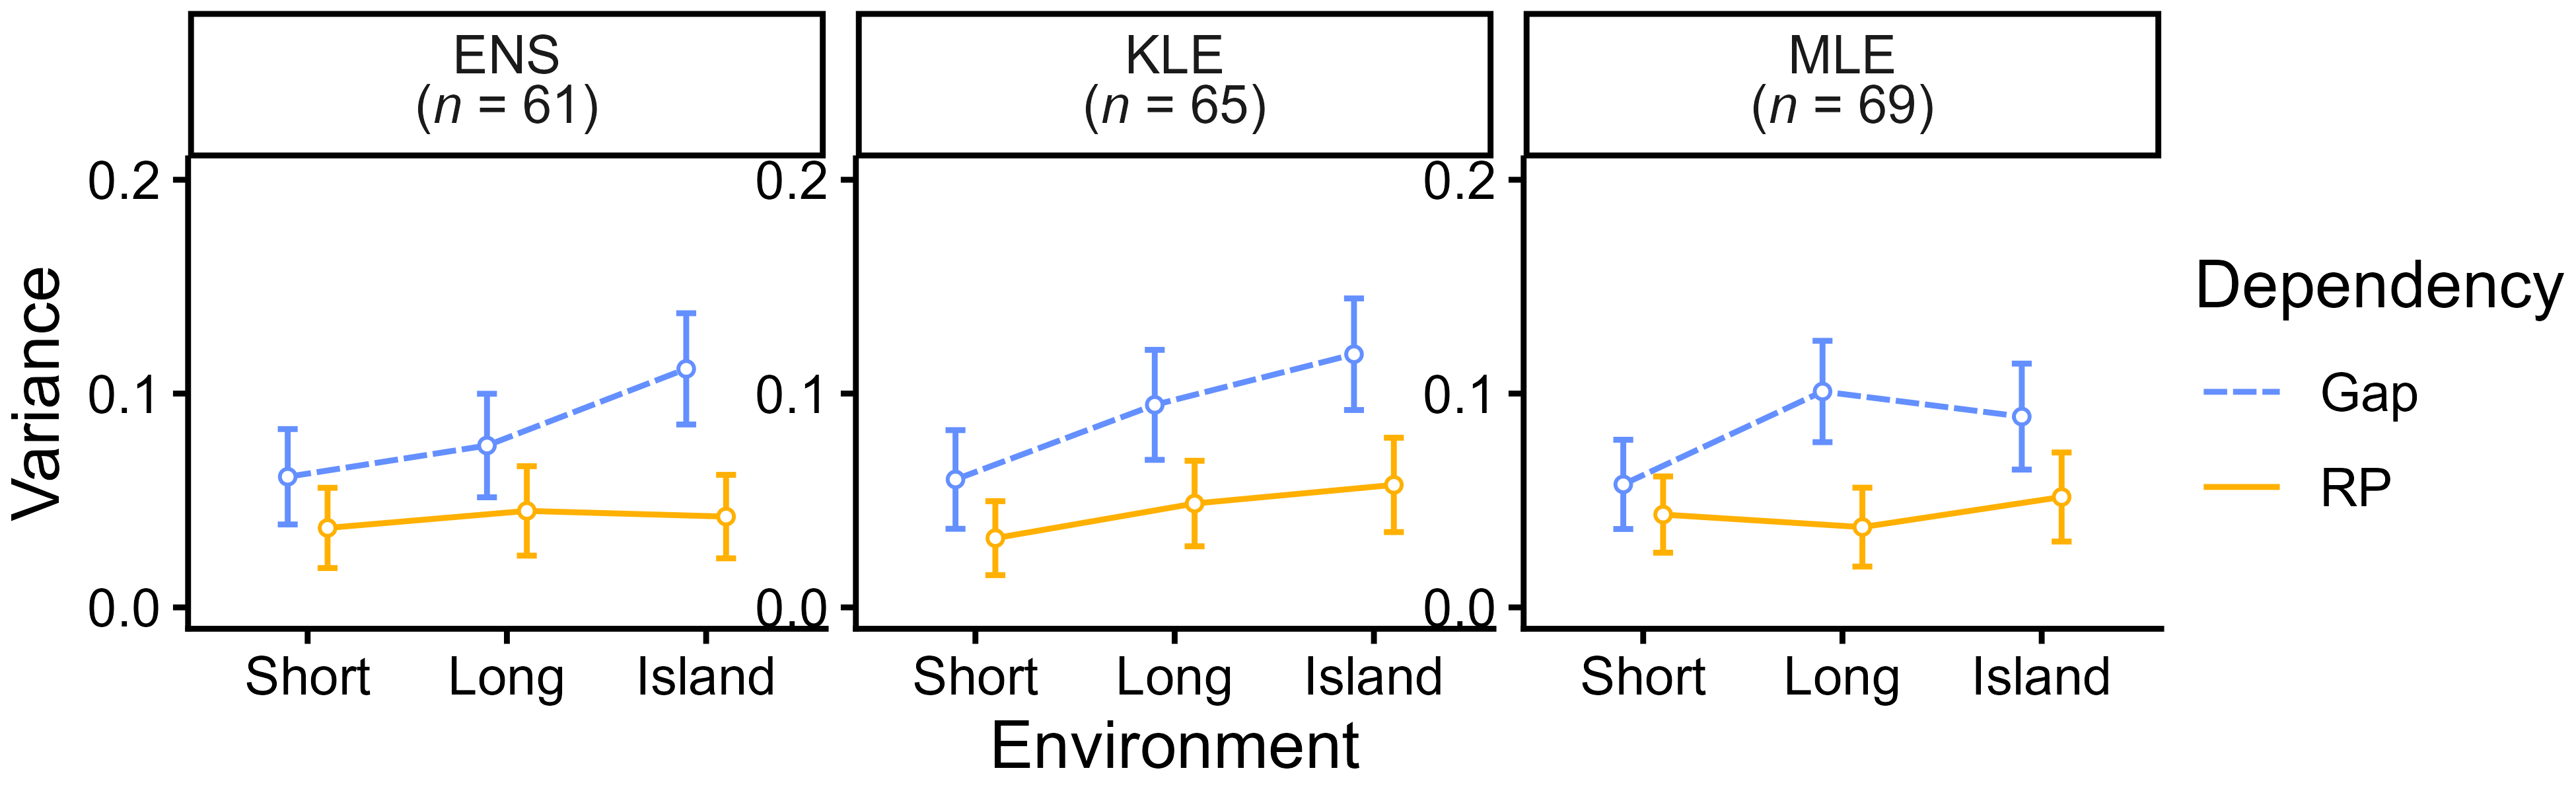
\includegraphics{../analysis/plots/src_spr_accuracy_var.png}
% \vspace{-12pt}
% \end{figure}

% ORC Model
\DTLloaddb{dt-orc-spr-var-model}{../analysis/tables/orc_spr_var_model.csv}
\ExplSyntaxOn
\tl_clear:N \tblrbody
\tl_build_begin:N \tblrbody
\DTLforeach{dt-orc-spr-var-model}{\coli=Parameter,\colii=Estimate,\coliii=$SE$,\coliv=$t$,\colv=$p$}{\tl_build_put_right:Ne \tblrbody {\exp_not:V \coli & \exp_not:V \colii & \exp_not:V \coliii & \exp_not:V \coliv & \exp_not:V \colv\\}}
\tl_build_end:N \tblrbody
\ExplSyntaxOff
\begin{longtblr}[caption={Summary of linear mixed-effects model on variance for comprehension-question accuracy in the ORC self-paced reading task}, label={tblr:app-orc-spr-var-model}, expand=\tblrbody, remark{Note}={Model formula: Model formula: Variance \~{} Dependency * Environment * Group + (1 + Dependency + Environment | Participant); reference level: Gap + Short + KE; estimate unit: variance; intercept: grand mean.}]{colspec={lX[r]X[r]X[r]X[r]}}\toprule
Parameter & Estimate~($\hat{\beta}$) & \textit{SE} & $t$ & $p$\\\midrule
\tblrbody\bottomrule
\end{longtblr}
\vspace{-12pt}

% ORC Posthoc
\DTLloaddb{dt-orc-spr-var-posthoc}{../analysis/tables/orc_spr_var_posthoc.csv}
\ExplSyntaxOn
\tl_clear:N \tblrbody
\tl_build_begin:N \tblrbody
\DTLforeach{dt-orc-spr-var-posthoc}{\coli=Group,\colii=Environment,\coliii=Contrast,\coliv=Estimate,\colv=$SE$,\colvi=$t$,\colvii=$p$}{\tl_build_put_right:Ne \tblrbody {\exp_not:V \coli & \exp_not:V \colii & \exp_not:V \coliii & \exp_not:V \coliv & \exp_not:V \colv & \exp_not:V \colvi & \exp_not:V \colvii\\}}
\tl_build_end:N \tblrbody
\ExplSyntaxOff
\begin{longtblr}[caption={Post-hoc tests on variance for comprehension-question accuracy in the ORC self-paced reading task}, label={tblr:app-orc-spr-var-posthoc}, expand=\tblrbody, remark{Note}={Adjustment to $p$-values done via multiple $t$ method for 9 tests.}]{colspec={XXXX[r]X[r]X[r]X[r]}}\toprule
Group & Environment & Contrast & Estimate~($\hat{\beta}$) & \textit{SE} & $t$ & $p$\\\midrule
\tblrbody\bottomrule
\end{longtblr}
\vspace{-12pt}

% SRC Model
\DTLloaddb{dt-src-spr-var-model}{../analysis/tables/src_spr_var_model.csv}
\ExplSyntaxOn
\tl_clear:N \tblrbody
\tl_build_begin:N \tblrbody
\DTLforeach{dt-src-spr-var-model}{\coli=Parameter,\colii=Estimate,\coliii=$SE$,\coliv=$t$,\colv=$p$}{\tl_build_put_right:Ne \tblrbody {\exp_not:V \coli & \exp_not:V \colii & \exp_not:V \coliii & \exp_not:V \coliv & \exp_not:V \colv\\}}
\tl_build_end:N \tblrbody
\ExplSyntaxOff
\begin{longtblr}[caption={Summary of linear mixed-effects model on variance for comprehension-question accuracy in the SRC self-paced reading task}, label={tblr:app-src-spr-var-model}, expand=\tblrbody, remark{Note}={Model formula: Model formula: Variance \~{} Dependency * Environment * Group + (1 + Dependency + Environment | Participant); reference level: Gap + Short + KE; estimate unit: variance; intercept: grand mean.}]{colspec={lX[r]X[r]X[r]X[r]}}\toprule
Parameter & Estimate~($\hat{\beta}$) & \textit{SE} & $t$ & $p$\\\midrule
\tblrbody\bottomrule
\end{longtblr}
\vspace{-12pt}

% SRC Posthoc
\DTLloaddb{dt-src-spr-var-posthoc}{../analysis/tables/src_spr_var_posthoc.csv}
\ExplSyntaxOn
\tl_clear:N \tblrbody
\tl_build_begin:N \tblrbody
\DTLforeach{dt-src-spr-var-posthoc}{\coli=Group,\colii=Environment,\coliii=Contrast,\coliv=Estimate,\colv=$SE$,\colvi=$t$,\colvii=$p$}{\tl_build_put_right:Ne \tblrbody {\exp_not:V \coli & \exp_not:V \colii & \exp_not:V \coliii & \exp_not:V \coliv & \exp_not:V \colv & \exp_not:V \colvi & \exp_not:V \colvii\\}}
\tl_build_end:N \tblrbody
\ExplSyntaxOff
\begin{longtblr}[caption={Post-hoc tests on variance for comprehension-question accuracy in the SRC self-paced reading task}, label={tblr:app-src-spr-var-posthoc}, expand=\tblrbody, remark{Note}={Adjustment to $p$-values done via multiple $t$ method for 9 tests.}]{colspec={XXXX[r]X[r]X[r]X[r]}}\toprule
Group & Environment & Contrast & Estimate~($\hat{\beta}$) & \textit{SE} & $t$ & $p$\\\midrule
\tblrbody\bottomrule
\end{longtblr}
\vspace{-12pt}

%========================================================%
\section{Proficiency effects for the SPRT variance data}\label{app-var-spr-proficiency}
%========================================================%

% ORC Figure
% \begin{figure}
% \caption{L2 proficiency effects on variance for comprehension-question accuracy in the ORC self-paced reading task} \label{fig:app-orc-spr-var-proficiency}
% \raggedright\setstretch{1}
% 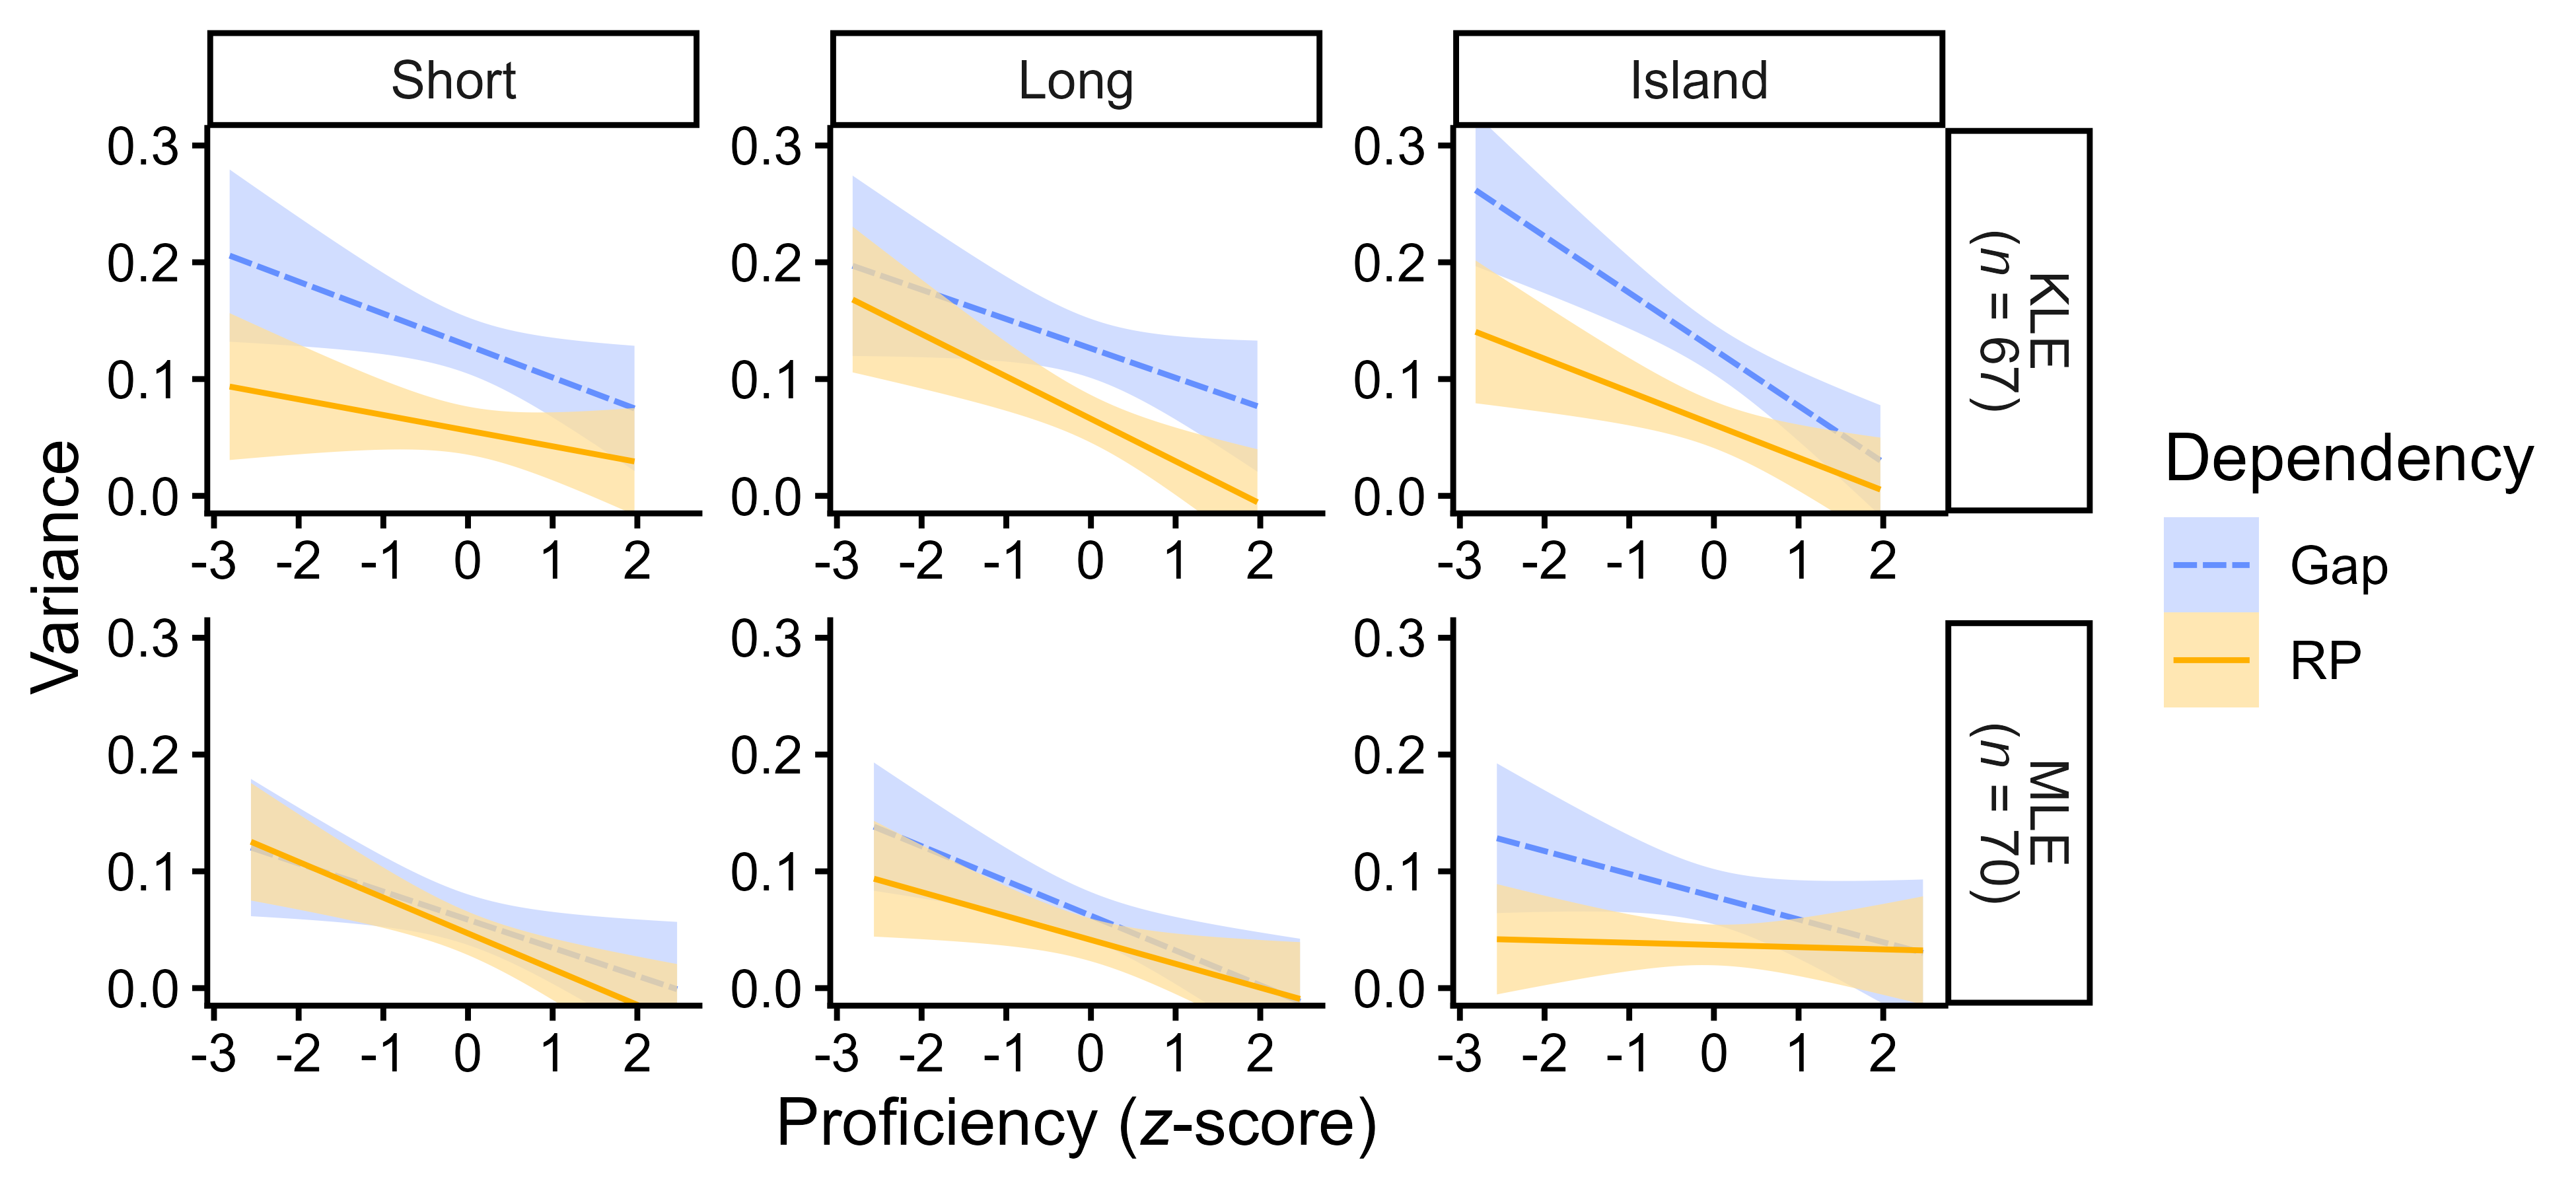
\includegraphics{../analysis/plots/orc_spr_var_proficiency.png}
% \vspace{-12pt}
% \end{figure}

% SRC Figure
% \begin{figure}
% \caption{L2 proficiency effects on variance for comprehension-question accuracy in the SRC self-paced reading task} \label{fig:app-src-spr-var-proficiency}
% \raggedright\setstretch{1}
% 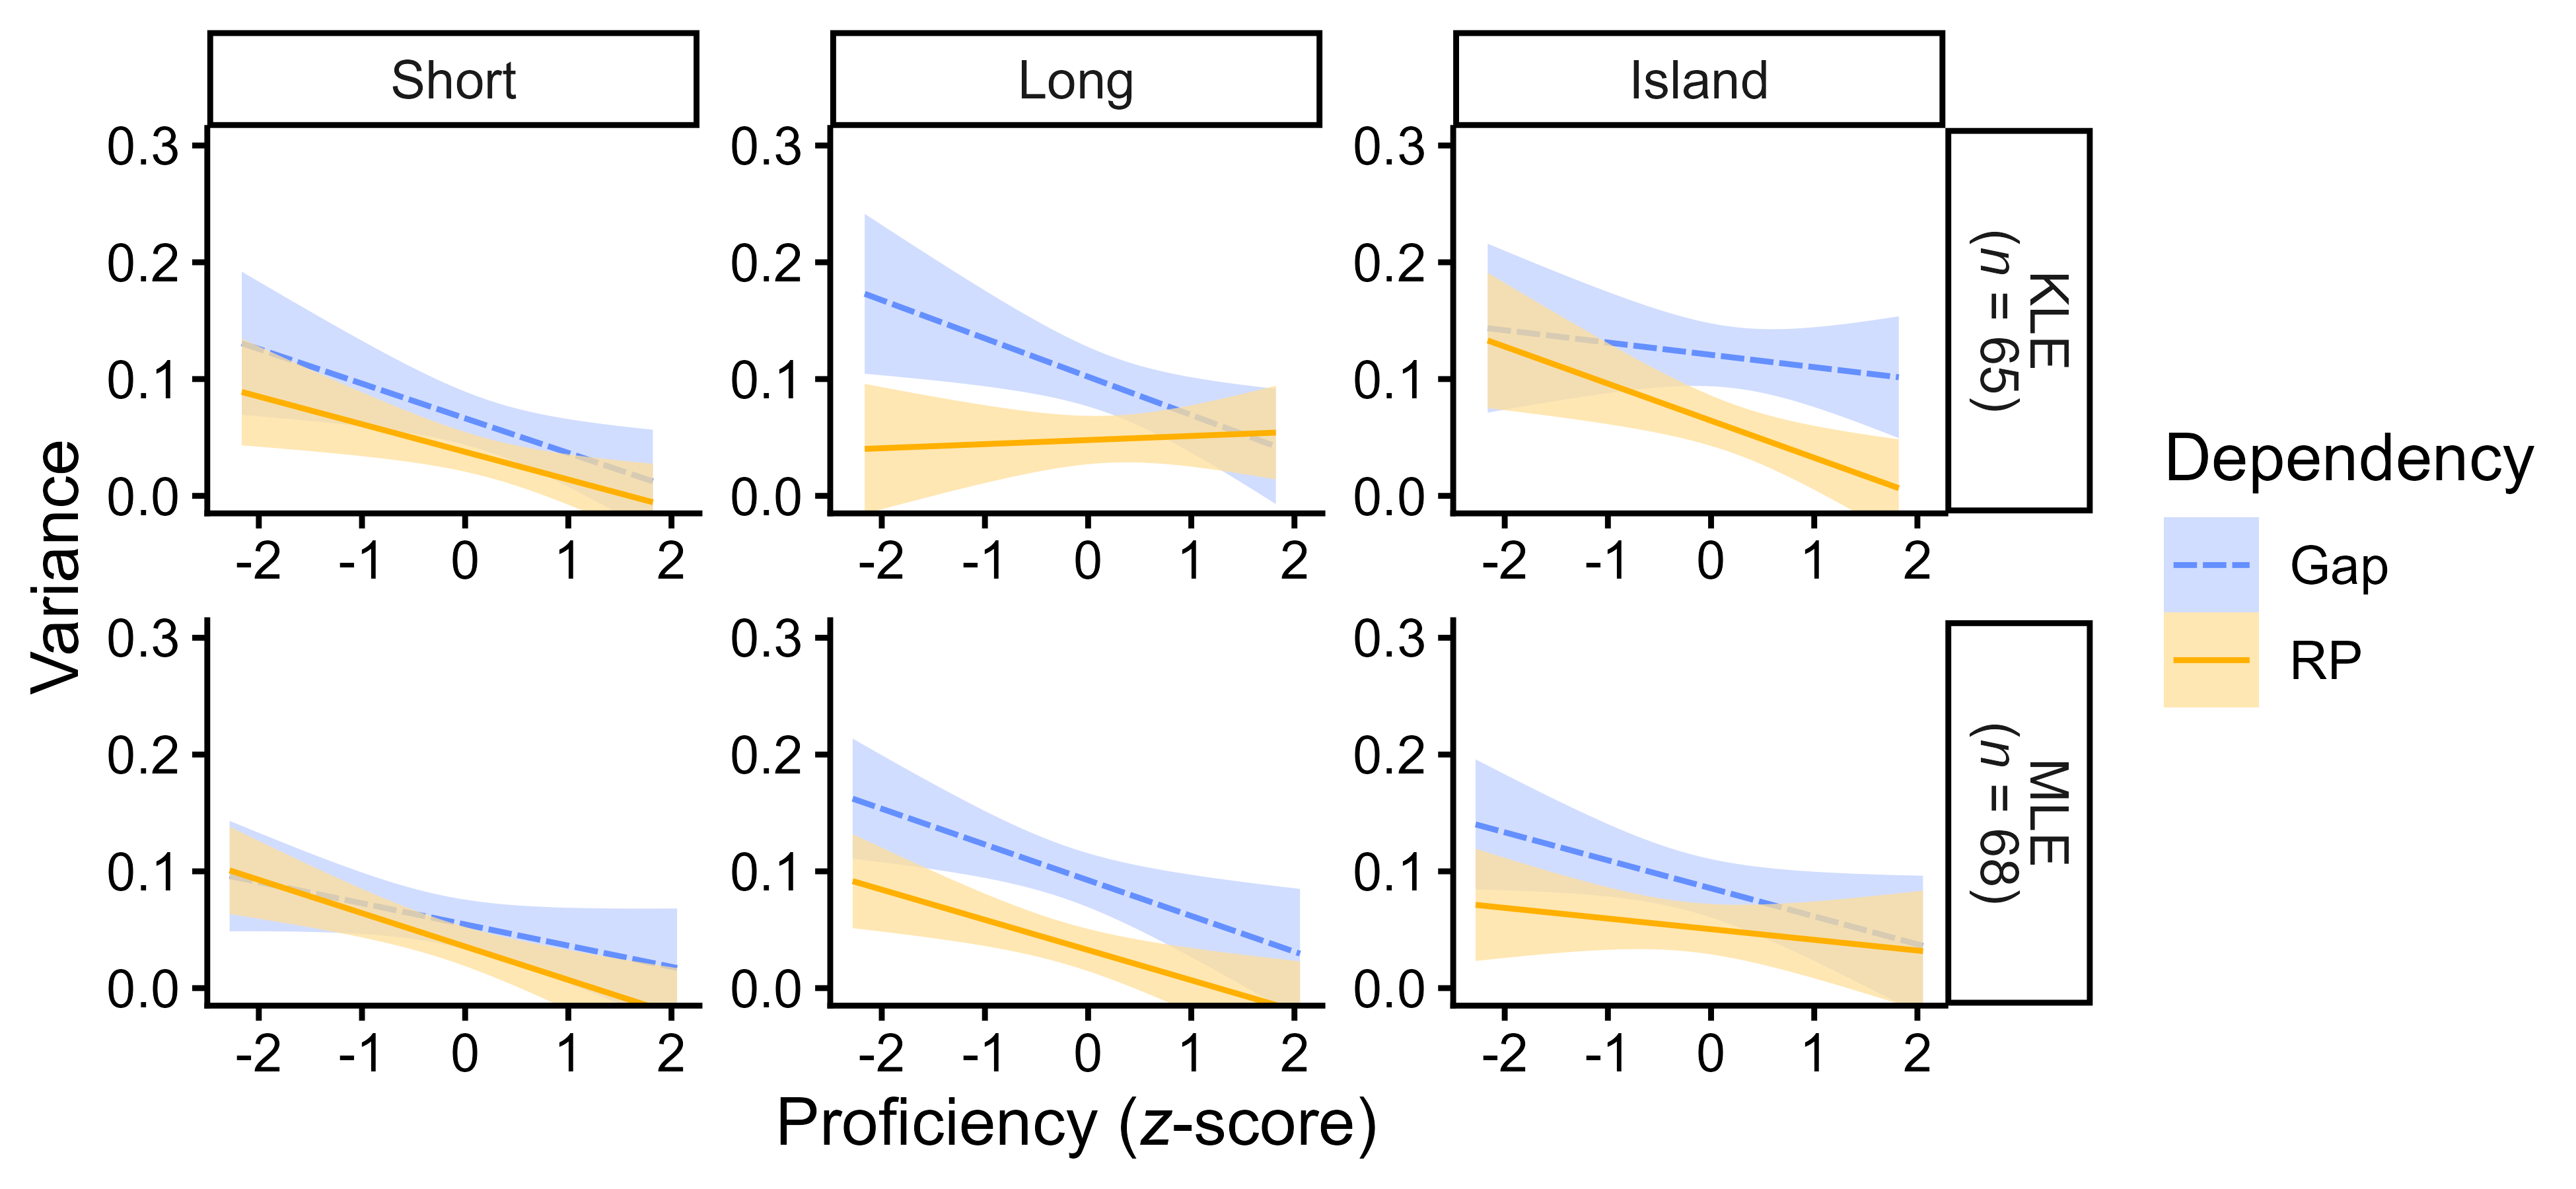
\includegraphics{../analysis/plots/src_spr_var_proficiency.png}
% \vspace{-12pt}
% \end{figure}

% ORC Model
\DTLloaddb{dt-orc-spr-var-proficiency-model}{../analysis/tables/orc_spr_var_proficiency_model.csv}
\ExplSyntaxOn
\tl_clear:N \tblrbody
\tl_build_begin:N \tblrbody
\DTLforeach{dt-orc-spr-var-proficiency-model}{\coli=Parameter,\colii=Estimate,\coliii=$SE$,\coliv=$t$,\colv=$p$}{\tl_build_put_right:Ne \tblrbody {\exp_not:V \coli & \exp_not:V \colii & \exp_not:V \coliii & \exp_not:V \coliv & \exp_not:V \colv\\}}
\tl_build_end:N \tblrbody
\ExplSyntaxOff
\begin{longtblr}[caption={Summary of linear mixed-effects model on L2 proficiency effects for variance in comprehension-question accuracy in the ORC self-paced reading task}, label={tblr:app-orc-spr-var-proficiency-model}, expand=\tblrbody, remark{Note}={Model formula: Model formula: Variance \~{} Dependency * Environment * Group * Proficiency + (1 + Dependency | Participant); reference level: Gap + Short + KE; estimate unit: variance; intercept: grand mean.}]{colspec={lX[r]X[r]X[r]X[r]}}\toprule
Parameter & Estimate~($\hat{\beta}$) & \textit{SE} & $t$ & $p$\\\midrule
\tblrbody\bottomrule
\end{longtblr}
\vspace{-12pt}

% ORC Posthoc
\DTLloaddb{dt-orc-spr-var-proficiency-posthoc}{../analysis/tables/orc_spr_var_proficiency_posthoc.csv}
\ExplSyntaxOn
\tl_clear:N \tblrbody
\tl_build_begin:N \tblrbody
\DTLforeach{dt-orc-spr-var-proficiency-posthoc}{\coli=Group,\colii=Environment,\coliii=Contrast,\coliv=Estimate,\colv=$SE$,\colvi=$t$,\colvii=$p$}{\tl_build_put_right:Ne \tblrbody {\exp_not:V \coli & \exp_not:V \colii & \exp_not:V \coliii & \exp_not:V \coliv & \exp_not:V \colv & \exp_not:V \colvi & \exp_not:V \colvii\\}}
\tl_build_end:N \tblrbody
\ExplSyntaxOff
\begin{longtblr}[caption={Post-hoc tests on L2 proficiency effects for variance in comprehension-question accuracy in the ORC self-paced reading task}, label={tblr:app-orc-spr-var-proficiency-posthoc}, expand=\tblrbody, remark{Note}={Adjustment to $p$-values done via multiple $t$ method for 6 tests.}]{colspec={XXXX[r]X[r]X[r]X[r]}}\toprule
Group & Environment & Contrast & Estimate~($\hat{\beta}$) & \textit{SE} & $t$ & $p$\\\midrule
\tblrbody\bottomrule
\end{longtblr}
\vspace{-12pt}

% SRC Model
\DTLloaddb{dt-src-spr-var-proficiency-model}{../analysis/tables/src_spr_var_proficiency_model.csv}
\ExplSyntaxOn
\tl_clear:N \tblrbody
\tl_build_begin:N \tblrbody
\DTLforeach{dt-src-spr-var-proficiency-model}{\coli=Parameter,\colii=Estimate,\coliii=$SE$,\coliv=$t$,\colv=$p$}{\tl_build_put_right:Ne \tblrbody {\exp_not:V \coli & \exp_not:V \colii & \exp_not:V \coliii & \exp_not:V \coliv & \exp_not:V \colv\\}}
\tl_build_end:N \tblrbody
\ExplSyntaxOff
\begin{longtblr}[caption={Summary of linear mixed-effects model on L2 proficiency effects for variance in comprehension-question accuracy in the SRC self-paced reading task}, label={tblr:app-src-spr-var-proficiency-model}, expand=\tblrbody, remark{Note}={Model formula: Model formula: Variance \~{} Dependency * Environment * Group * Proficiency + (1 + Dependency + Environment | Participant); reference level: Gap + Short + KE; estimate unit: variance; intercept: grand mean.}]{colspec={lX[r]X[r]X[r]X[r]}}\toprule
Parameter & Estimate~($\hat{\beta}$) & \textit{SE} & $t$ & $p$\\\midrule
\tblrbody\bottomrule
\end{longtblr}
\vspace{-12pt}

% SRC Posthoc
\DTLloaddb{dt-src-spr-var-proficiency-posthoc}{../analysis/tables/src_spr_var_proficiency_posthoc.csv}
\ExplSyntaxOn
\tl_clear:N \tblrbody
\tl_build_begin:N \tblrbody
\DTLforeach{dt-src-spr-var-proficiency-posthoc}{\coli=Group,\colii=Environment,\coliii=Contrast,\coliv=Estimate,\colv=$SE$,\colvi=$t$,\colvii=$p$}{\tl_build_put_right:Ne \tblrbody {\exp_not:V \coli & \exp_not:V \colii & \exp_not:V \coliii & \exp_not:V \coliv & \exp_not:V \colv & \exp_not:V \colvi & \exp_not:V \colvii\\}}
\tl_build_end:N \tblrbody
\ExplSyntaxOff
\begin{longtblr}[caption={Post-hoc tests on L2 proficiency effects for variance in comprehension-question accuracy in the SRC self-paced reading task}, label={tblr:app-src-spr-var-proficiency-posthoc}, expand=\tblrbody, remark{Note}={Adjustment to $p$-values done via multiple $t$ method for 6 tests.}]{colspec={XXXX[r]X[r]X[r]X[r]}}\toprule
Group & Environment & Contrast & Estimate~($\hat{\beta}$) & \textit{SE} & $t$ & $p$\\\midrule
\tblrbody\bottomrule
\end{longtblr}
\vspace{-12pt}

%========================================================%
\section{AJT variance data}\label{app-var-ajt}
%========================================================%

% ORC Means
% \DTLloaddb{dt-ajt-var}{../analysis/tables/ajt_var.csv}
% \ExplSyntaxOn
% \tl_clear:N \tblrbody
% \tl_build_begin:N \tblrbody
% \DTLforeach[\equal{\study}{ORC}]{dt-ajt-var}{\study=study,\coli=Pairing,\colii=Dependency,\coliii=Environment,\coliv=Mean,\colv=$CI$}{\tl_build_put_right:Ne \tblrbody {\exp_not:V \coli & \exp_not:V \colii & \exp_not:V \coliii & \exp_not:V \coliv & \exp_not:V \colv\\}}
% \tl_build_end:N \tblrbody
% \ExplSyntaxOff
% \begin{longtblr}[caption={Variance for acceptance in the ORC acceptability judgment task}, label={tblr:app-orc-ajt-var}, expand=\tblrbody]{colspec={XXXX[r]X[r]}}\toprule
% Pairing & Dependency & Environment & Mean & 95\% \textit{CI}\\\midrule
% \tblrbody\bottomrule
% \end{longtblr}
% \vspace{-12pt}

% SRC Means
% \ExplSyntaxOn
% \tl_clear:N \tblrbody
% \tl_build_begin:N \tblrbody
% \DTLforeach[\equal{\study}{SRC}]{dt-ajt-var}{\study=study,\coli=Pairing,\colii=Dependency,\coliii=Environment,\coliv=Mean,\colv=$CI$}{\tl_build_put_right:Ne \tblrbody {\exp_not:V \coli & \exp_not:V \colii & \exp_not:V \coliii & \exp_not:V \coliv & \exp_not:V \colv\\}}
% \tl_build_end:N \tblrbody
% \ExplSyntaxOff
% \begin{longtblr}[caption={Variance for acceptance in the SRC acceptability judgment task}, label={tblr:app-src-ajt-var}, expand=\tblrbody]{colspec={XXXX[r]X[r]}}\toprule
% Pairing & Dependency & Environment & Mean & 95\% \textit{CI}\\\midrule
% \tblrbody\bottomrule
% \end{longtblr}
% \vspace{-12pt}

% ORC Figure
% \begin{figure}
% \caption{Mean variance for acceptance in the ORC acceptability judgment task} \label{fig:app-orc-ajt-var}
% \raggedright\setstretch{1}
% 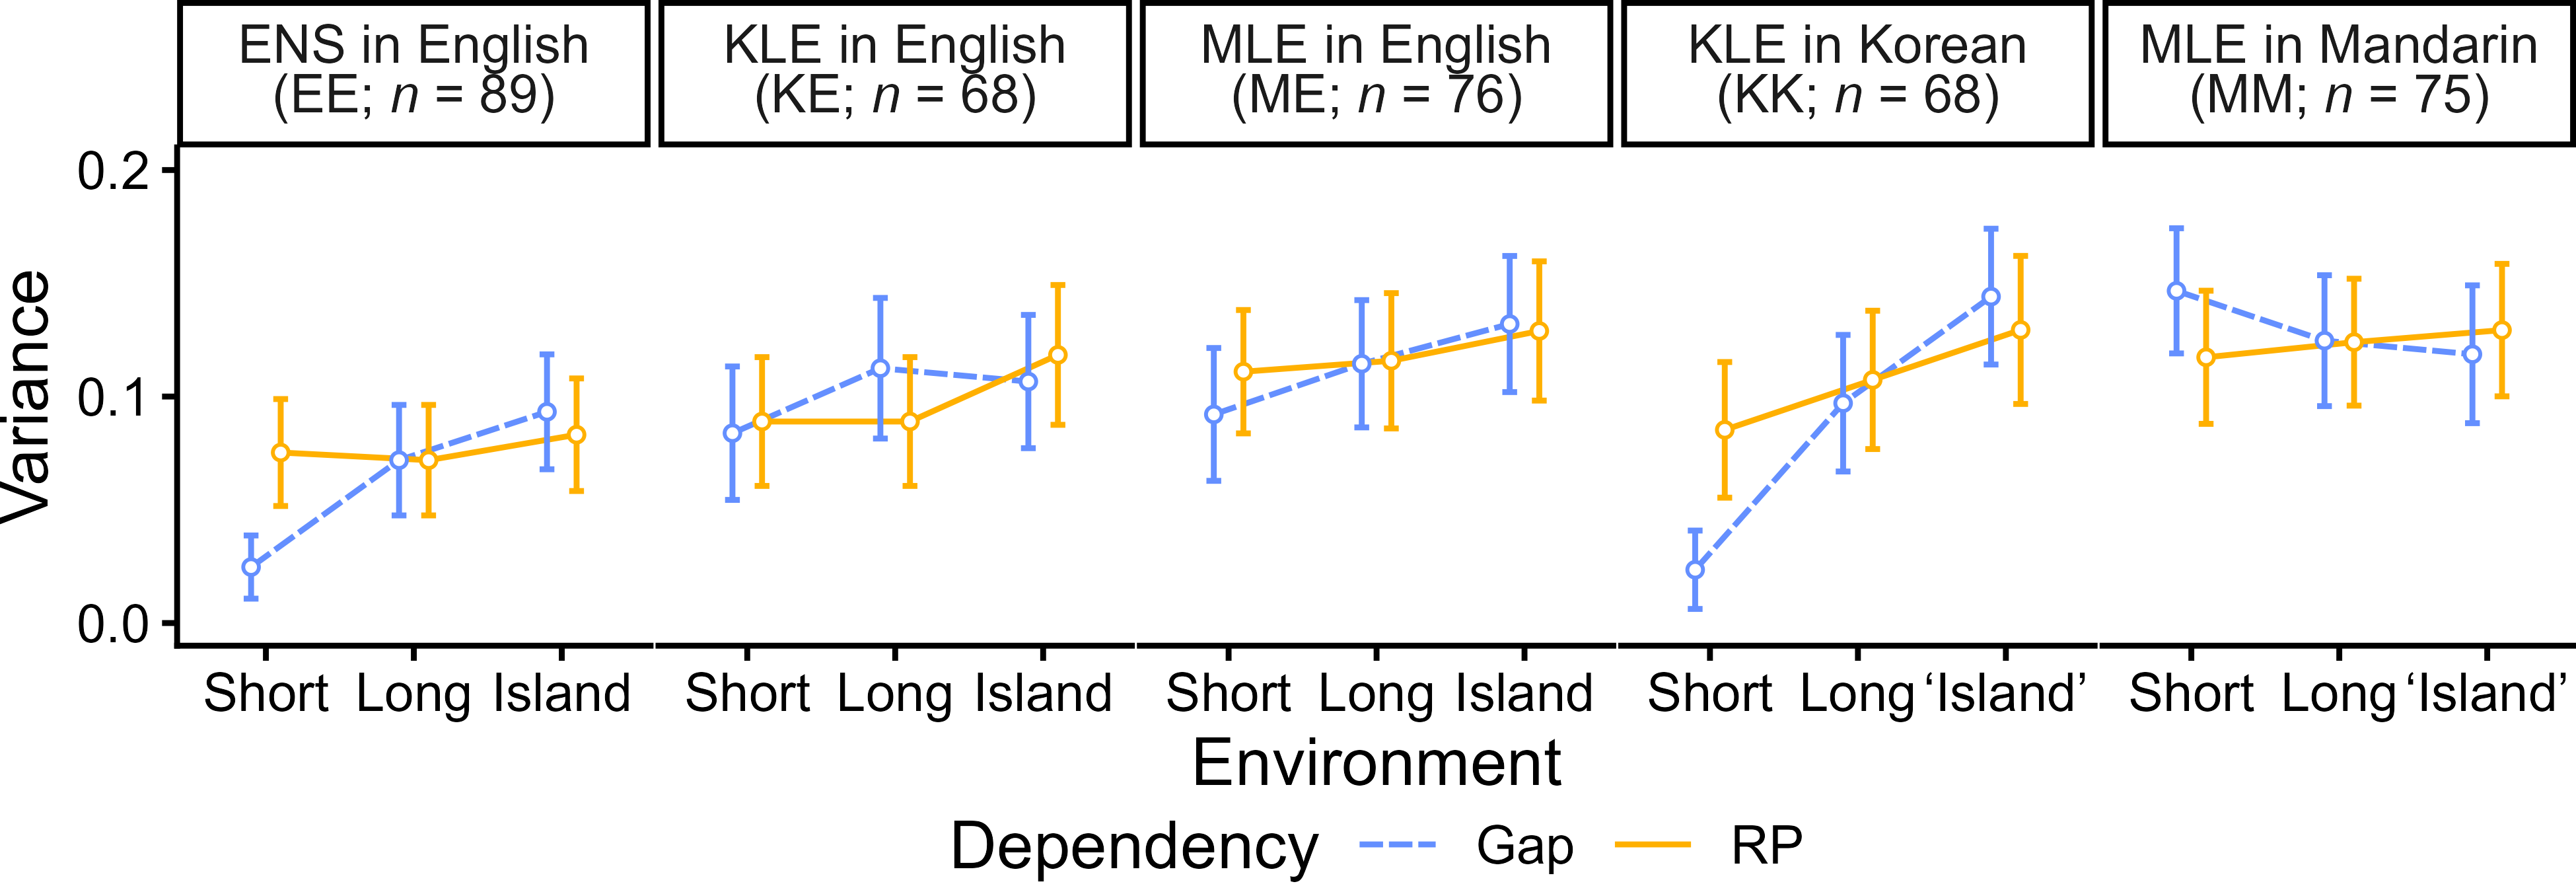
\includegraphics{../analysis/plots/orc_ajt_var.png}
% \vspace{-12pt}
% \end{figure}

% SRC Figure
% \begin{figure}
% \caption{Mean variance for acceptance in the SRC acceptability judgment task} \label{fig:app-src-ajt-var}
% \raggedright\setstretch{1}
% 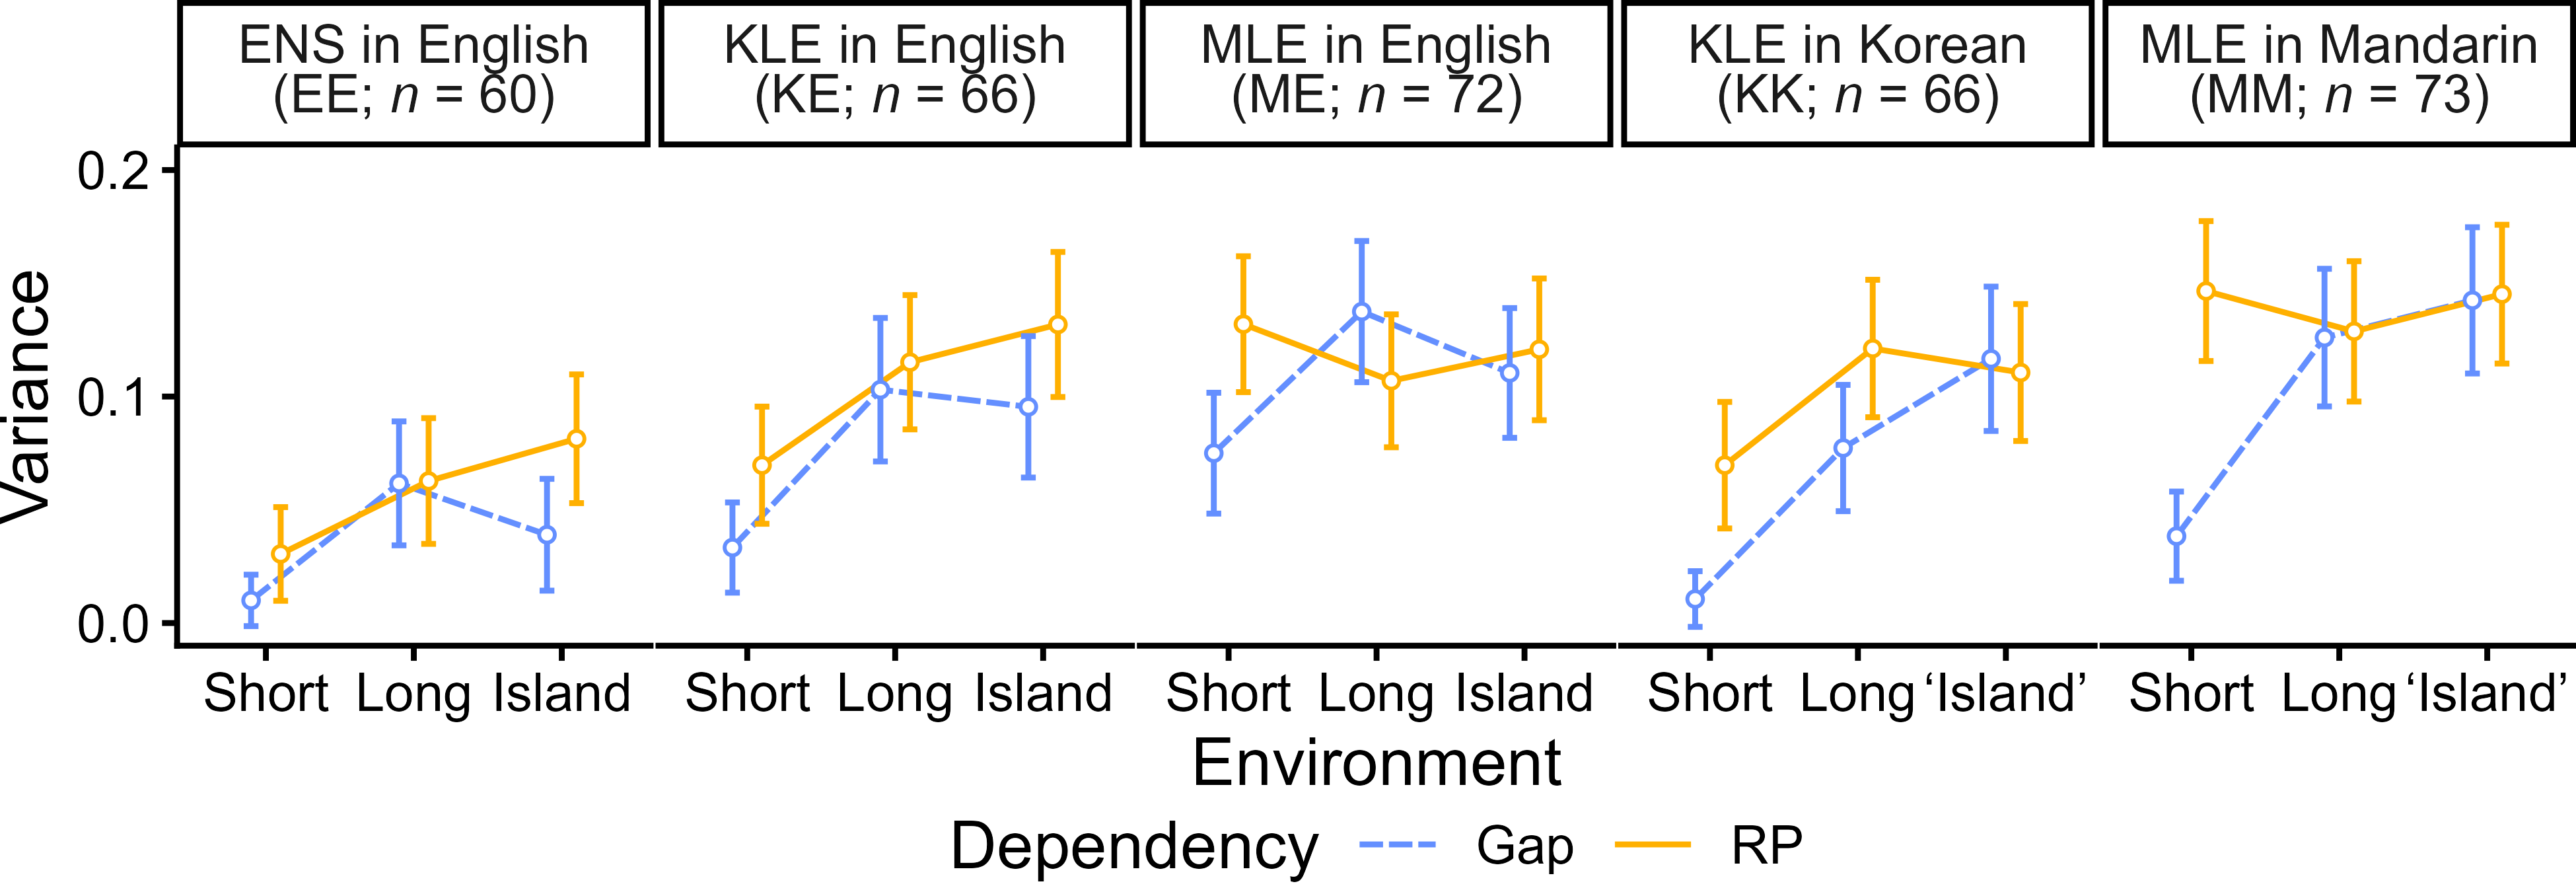
\includegraphics{../analysis/plots/src_ajt_var.png}
% \vspace{-12pt}
% \end{figure}

% ORC Model
\DTLloaddb{dt-orc-ajt-var-model}{../analysis/tables/orc_ajt_var_model.csv}
\ExplSyntaxOn
\tl_clear:N \tblrbody
\tl_build_begin:N \tblrbody
\DTLforeach{dt-orc-ajt-var-model}{\coli=Parameter,\colii=Estimate,\coliii=$SE$,\coliv=$t$,\colv=$p$}{\tl_build_put_right:Ne \tblrbody {\exp_not:V \coli & \exp_not:V \colii & \exp_not:V \coliii & \exp_not:V \coliv & \exp_not:V \colv\\}}
\tl_build_end:N \tblrbody
\ExplSyntaxOff
\begin{longtblr}[caption={Summary of linear mixed-effects model on variance for acceptance in the ORC acceptability judgment task}, label={tblr:app-orc-ajt-var-model}, expand=\tblrbody, remark{Note}={Model formula: Model formula: Variance \~{} Dependency * Environment * Pairing + (1 + Dependency * Environment | Participant); reference level: Gap + Short + KE; estimate unit: variance; intercept: grand mean.}]{colspec={lX[r]X[r]X[r]X[r]}}\toprule
Parameter & Estimate~($\hat{\beta}$) & \textit{SE} & $t$ & $p$\\\midrule
\tblrbody\bottomrule
\end{longtblr}
\vspace{-12pt}

% ORC Posthoc
\DTLloaddb{dt-orc-ajt-var-posthoc}{../analysis/tables/orc_ajt_var_posthoc.csv}
\ExplSyntaxOn
\tl_clear:N \tblrbody
\tl_build_begin:N \tblrbody
\DTLforeach{dt-orc-ajt-var-posthoc}{\coli=Pairing,\colii=Environment,\coliii=Contrast,\coliv=Estimate,\colv=$SE$,\colvi=$t$,\colvii=$p$}{\tl_build_put_right:Ne \tblrbody {\exp_not:V \coli & \exp_not:V \colii & \exp_not:V \coliii & \exp_not:V \coliv & \exp_not:V \colv & \exp_not:V \colvi & \exp_not:V \colvii\\}}
\tl_build_end:N \tblrbody
\ExplSyntaxOff
\begin{longtblr}[caption={Post-hoc tests on variance for acceptance in the ORC acceptability judgment task}, label={tblr:app-orc-ajt-var-posthoc}, expand=\tblrbody, remark{Note}={Adjustment to $p$-values done via multiple $t$ method for 15 tests.}]{colspec={XXXX[r]X[r]X[r]X[r]}}\toprule
Pairing & Environment & Contrast & Estimate~($\hat{\beta}$) & \textit{SE} & $t$ & $p$\\\midrule
\tblrbody\bottomrule
\end{longtblr}
\vspace{-12pt}

% SRC Model
\DTLloaddb{dt-src-ajt-var-model}{../analysis/tables/src_ajt_var_model.csv}
\ExplSyntaxOn
\tl_clear:N \tblrbody
\tl_build_begin:N \tblrbody
\DTLforeach{dt-src-ajt-var-model}{\coli=Parameter,\colii=Estimate,\coliii=$SE$,\coliv=$t$,\colv=$p$}{\tl_build_put_right:Ne \tblrbody {\exp_not:V \coli & \exp_not:V \colii & \exp_not:V \coliii & \exp_not:V \coliv & \exp_not:V \colv\\}}
\tl_build_end:N \tblrbody
\ExplSyntaxOff
\begin{longtblr}[caption={Summary of linear mixed-effects model on variance for acceptance in the SRC acceptability judgment task}, label={tblr:app-src-ajt-var-model}, expand=\tblrbody, remark{Note}={Model formula: Model formula: Variance \~{} Dependency * Environment * Pairing + (1 + Dependency * Environment | Participant); reference level: Gap + Short + KE; estimate unit: variance; intercept: grand mean.}]{colspec={lX[r]X[r]X[r]X[r]}}\toprule
Parameter & Estimate~($\hat{\beta}$) & \textit{SE} & $t$ & $p$\\\midrule
\tblrbody\bottomrule
\end{longtblr}
\vspace{-12pt}

% SRC Posthoc
\DTLloaddb{dt-src-ajt-var-posthoc}{../analysis/tables/src_ajt_var_posthoc.csv}
\ExplSyntaxOn
\tl_clear:N \tblrbody
\tl_build_begin:N \tblrbody
\DTLforeach{dt-src-ajt-var-posthoc}{\coli=Pairing,\colii=Environment,\coliii=Contrast,\coliv=Estimate,\colv=$SE$,\colvi=$t$,\colvii=$p$}{\tl_build_put_right:Ne \tblrbody {\exp_not:V \coli & \exp_not:V \colii & \exp_not:V \coliii & \exp_not:V \coliv & \exp_not:V \colv & \exp_not:V \colvi & \exp_not:V \colvii\\}}
\tl_build_end:N \tblrbody
\ExplSyntaxOff
\begin{longtblr}[caption={Post-hoc tests on variance for acceptance in the SRC acceptability judgment task}, label={tblr:app-src-ajt-var-posthoc}, expand=\tblrbody, remark{Note}={Adjustment to $p$-values done via multiple $t$ method for 15 tests.}]{colspec={XXXX[r]X[r]X[r]X[r]}}\toprule
Pairing & Environment & Contrast & Estimate~($\hat{\beta}$) & \textit{SE} & $t$ & $p$\\\midrule
\tblrbody\bottomrule
\end{longtblr}
\vspace{-12pt}

%========================================================%
\section{Proficiency effects for the AJT variance data}\label{app-var-ajt-proficiency}
%========================================================%

% ORC Figure
% \begin{figure}
% \caption{L2 proficiency effects on variance for acceptance in the ORC acceptability judgment task} \label{fig:app-orc-ajt-var-proficiency}
% \raggedright\setstretch{1}
% 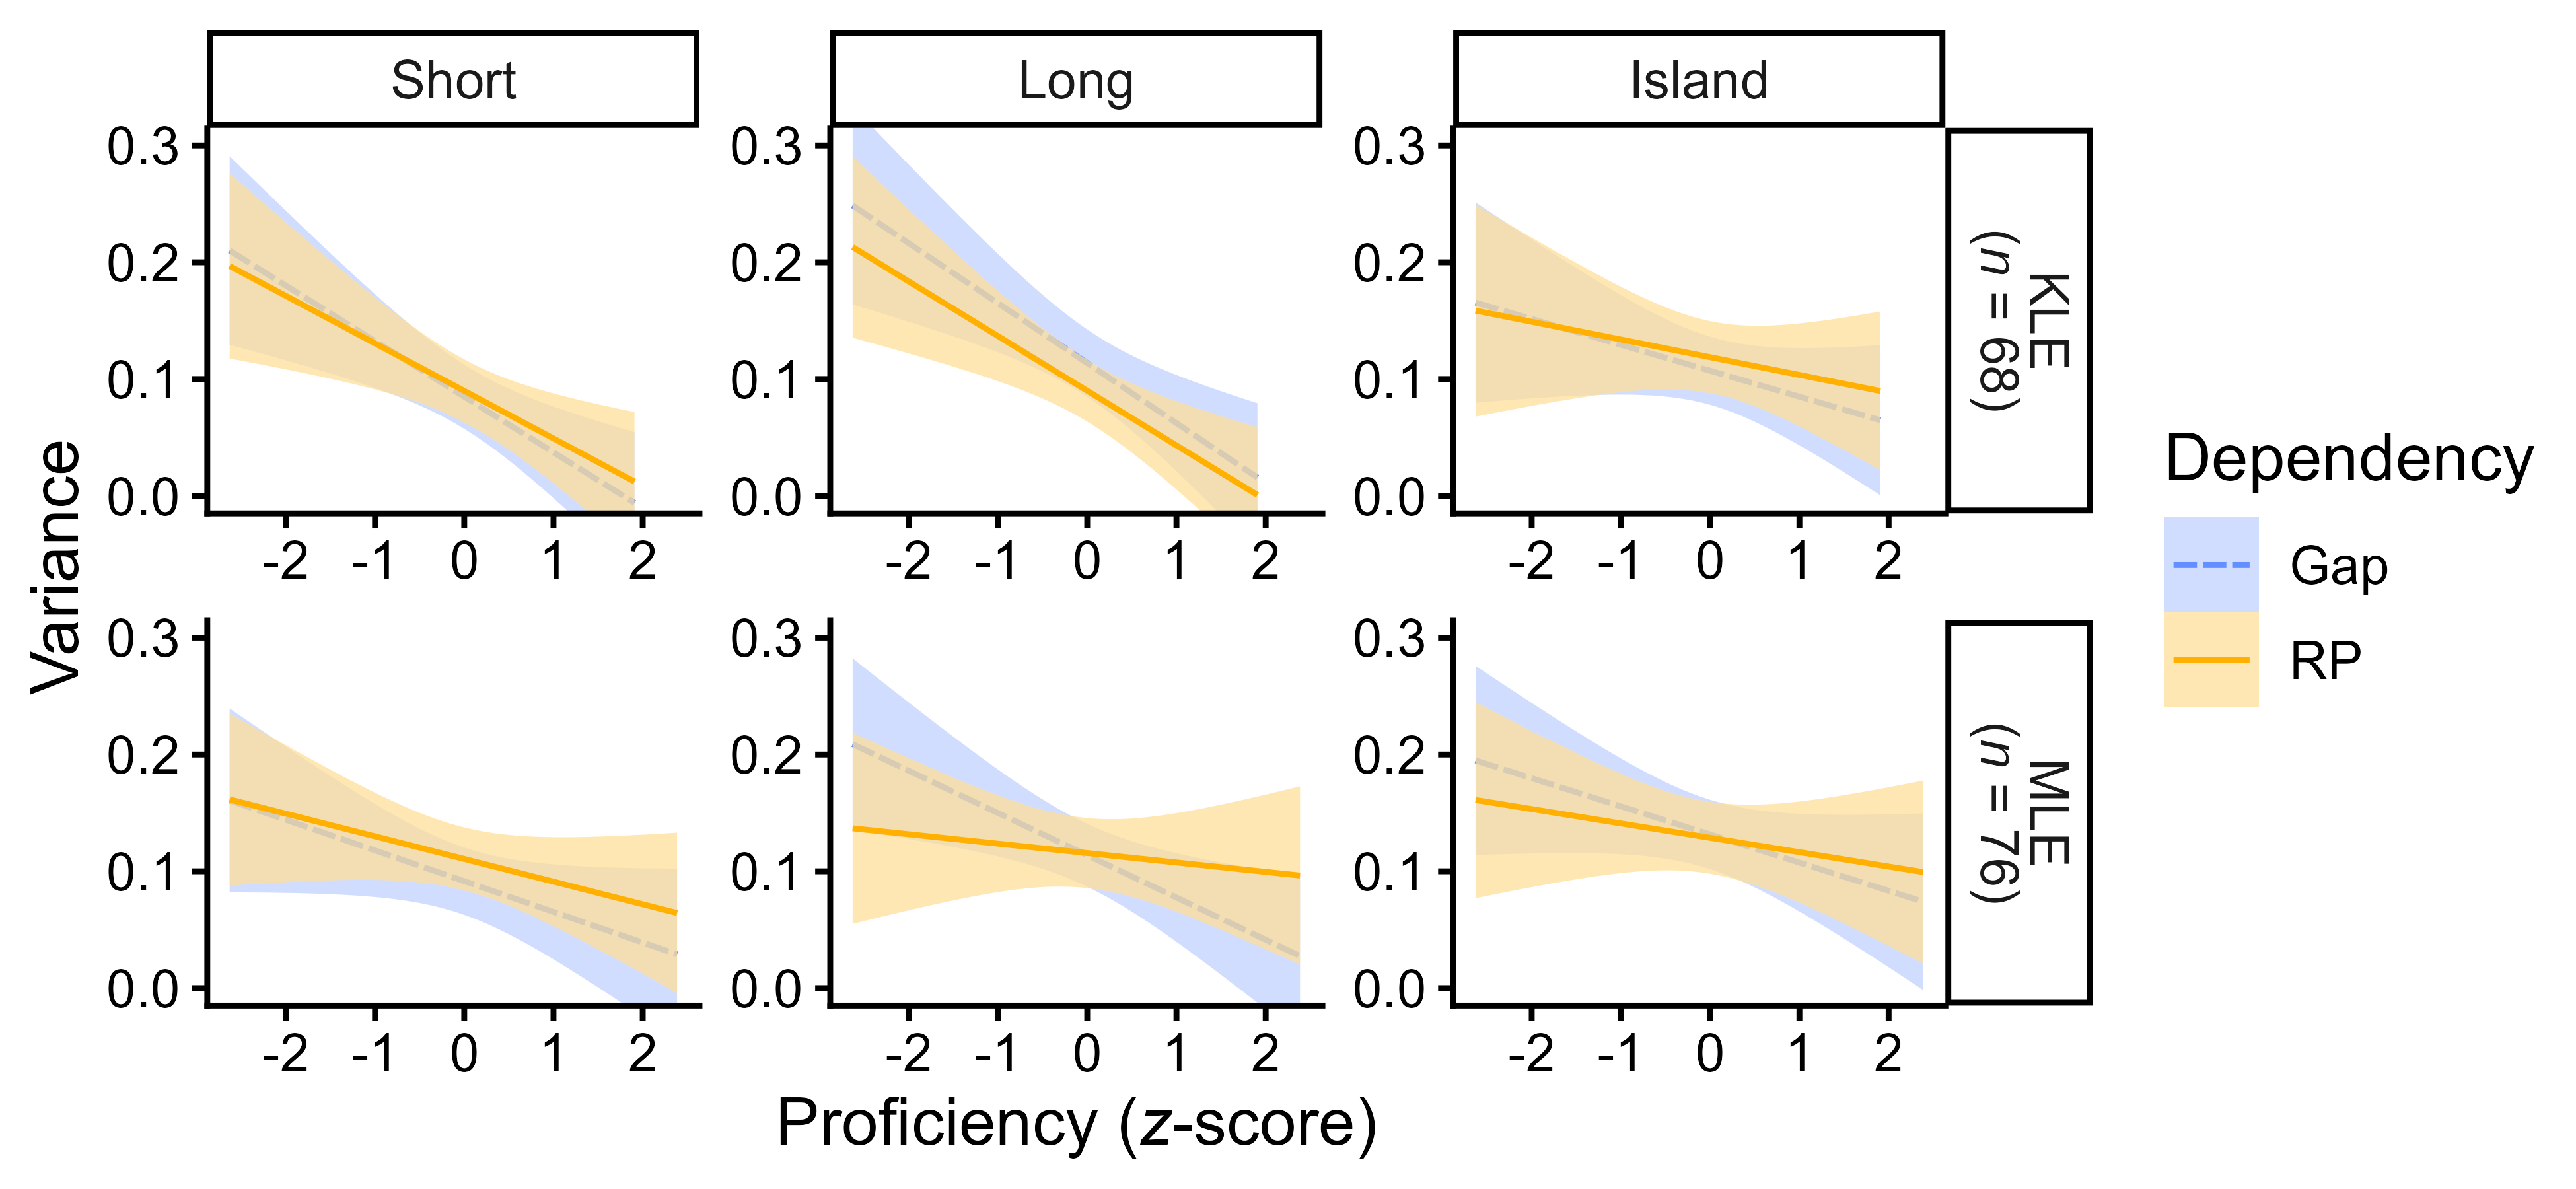
\includegraphics{../analysis/plots/orc_ajt_var_proficiency.png}
% \vspace{-12pt}
% \end{figure}

% SRC Figure
% \begin{figure}
% \caption{L2 proficiency effects on variance for acceptance in the SRC acceptability judgment task} \label{fig:app-src-ajt-var-proficiency}
% \raggedright\setstretch{1}
% 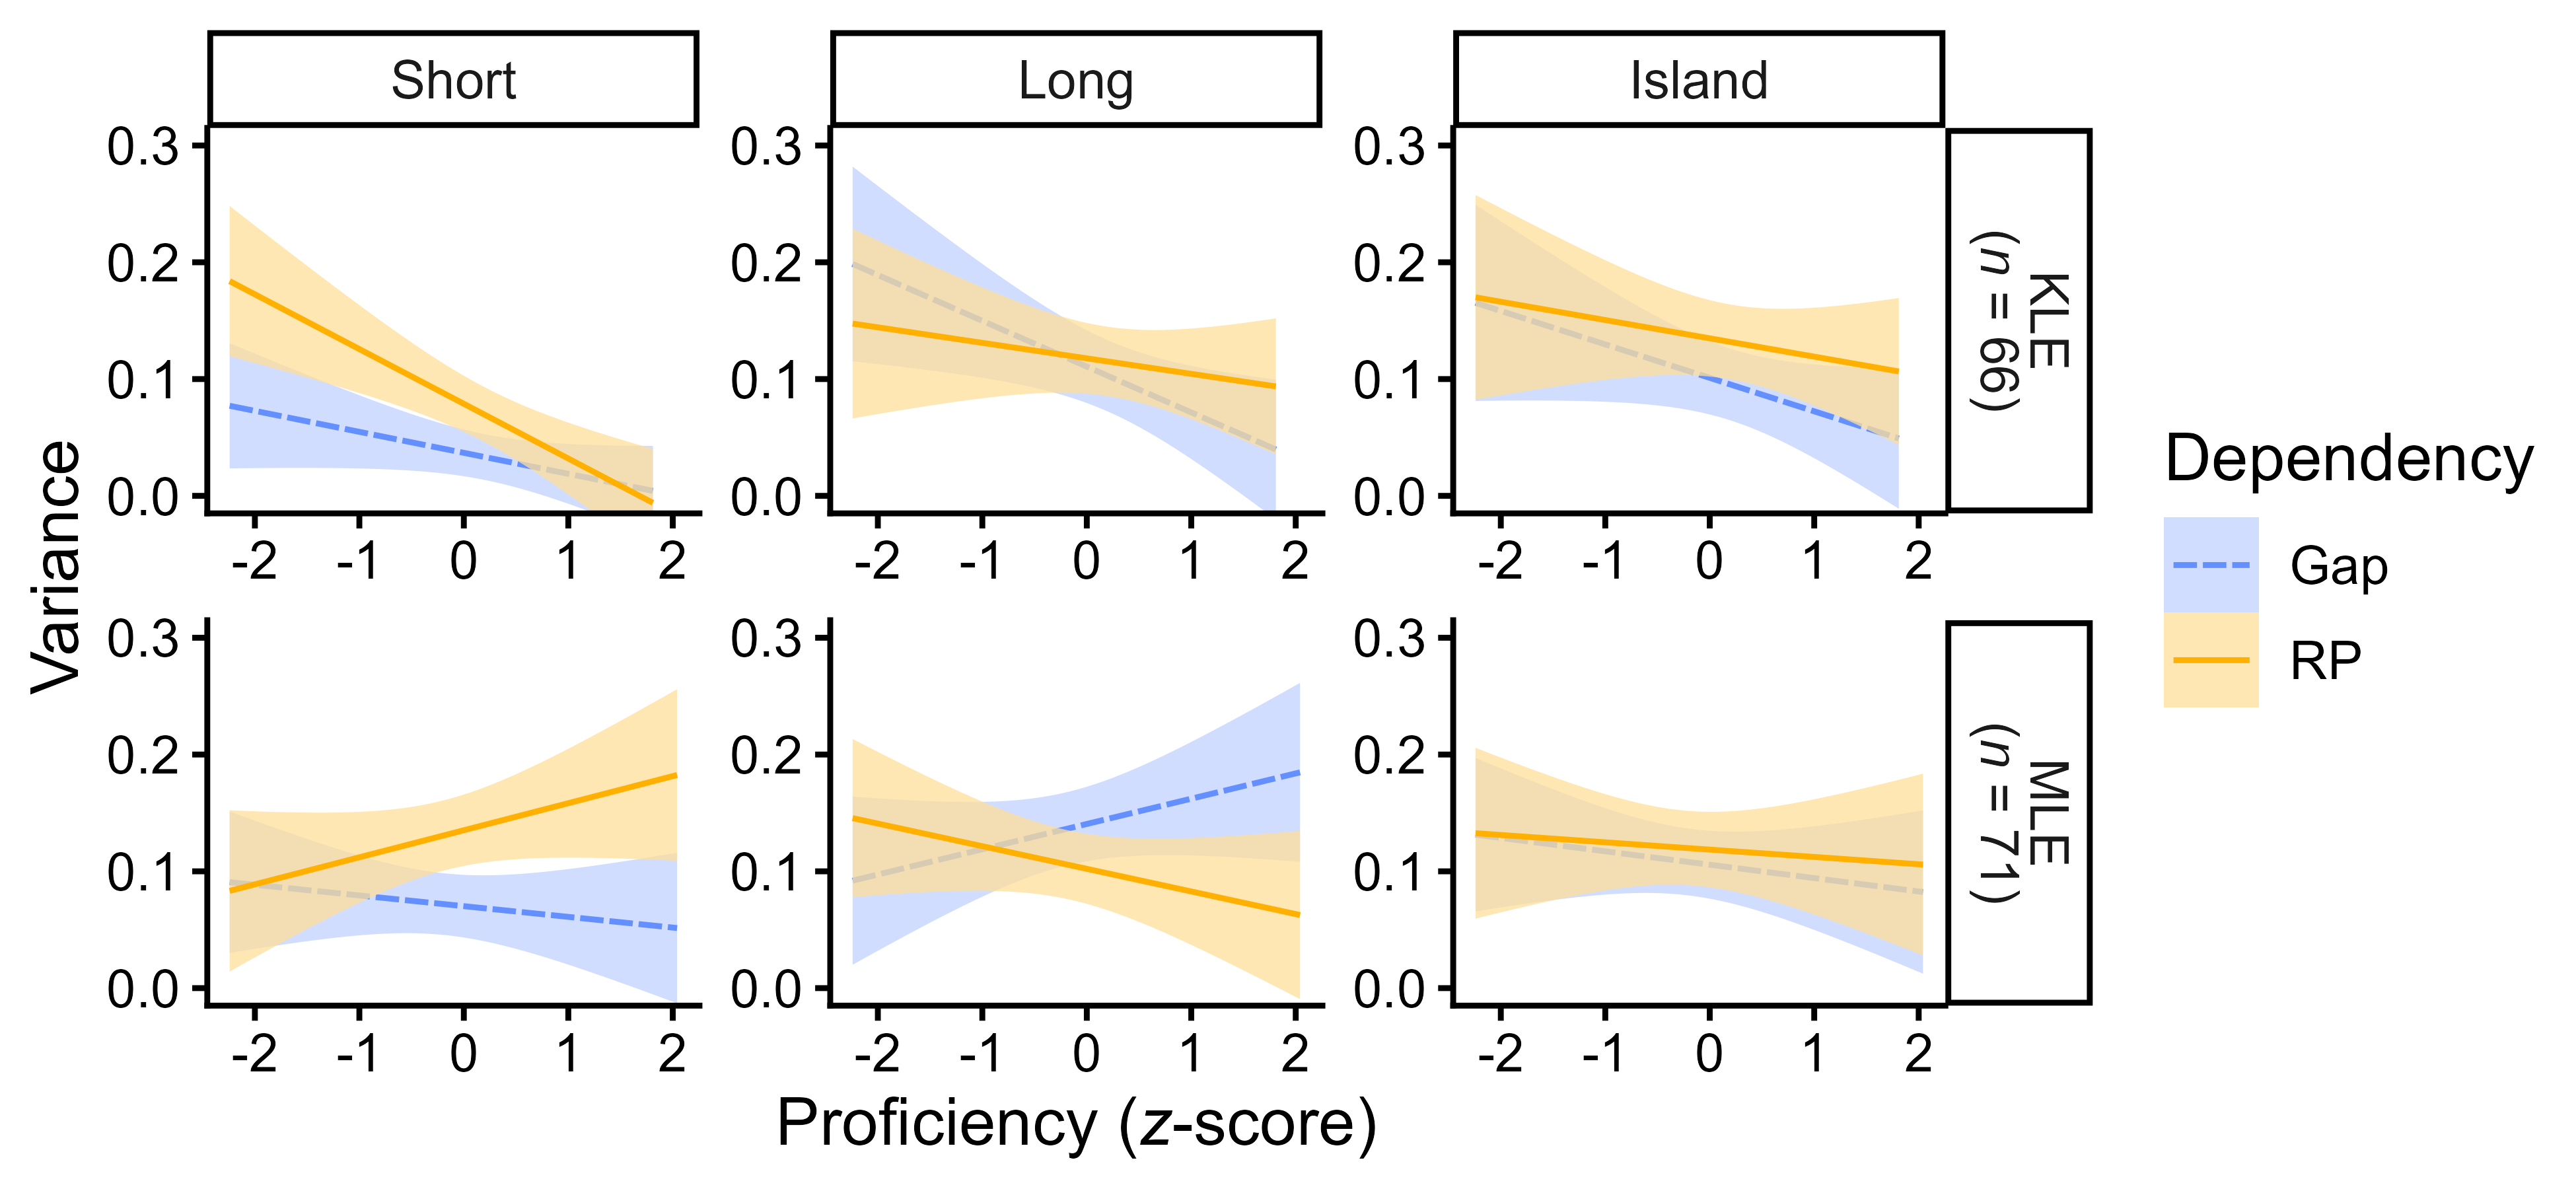
\includegraphics{../analysis/plots/src_ajt_var_proficiency.png}
% \vspace{-12pt}
% \end{figure}

% ORC Model
\DTLloaddb{dt-orc-ajt-var-proficiency-model}{../analysis/tables/orc_ajt_var_proficiency_model.csv}
\ExplSyntaxOn
\tl_clear:N \tblrbody
\tl_build_begin:N \tblrbody
\DTLforeach{dt-orc-ajt-var-proficiency-model}{\coli=Parameter,\colii=Estimate,\coliii=$SE$,\coliv=$t$,\colv=$p$}{\tl_build_put_right:Ne \tblrbody {\exp_not:V \coli & \exp_not:V \colii & \exp_not:V \coliii & \exp_not:V \coliv & \exp_not:V \colv\\}}
\tl_build_end:N \tblrbody
\ExplSyntaxOff
\begin{longtblr}[caption={Summary of linear mixed-effects model on L2 proficiency effects on variance for acceptance in the ORC acceptability judgment task}, label={tblr:app-orc-ajt-var-proficiency-model}, expand=\tblrbody, remark{Note}={Model formula: Model formula: Variance \~{} Dependency * Environment * Pairing * Proficiency + (1 + Dependency + Environment | Participant); reference level: Gap + Short + KE; estimate unit: variance; intercept: grand mean.}]{colspec={lX[r]X[r]X[r]X[r]}}\toprule
Parameter & Estimate~($\hat{\beta}$) & \textit{SE} & $t$ & $p$\\\midrule
\tblrbody\bottomrule
\end{longtblr}
\vspace{-12pt}

% ORC Posthoc
\DTLloaddb{dt-orc-ajt-var-proficiency-posthoc}{../analysis/tables/orc_ajt_var_proficiency_posthoc.csv}
\ExplSyntaxOn
\tl_clear:N \tblrbody
\tl_build_begin:N \tblrbody
\DTLforeach{dt-orc-ajt-var-proficiency-posthoc}{\coli=Pairing,\colii=Environment,\coliii=Contrast,\coliv=Estimate,\colv=$SE$,\colvi=$t$,\colvii=$p$}{\tl_build_put_right:Ne \tblrbody {\exp_not:V \coli & \exp_not:V \colii & \exp_not:V \coliii & \exp_not:V \coliv & \exp_not:V \colv & \exp_not:V \colvi & \exp_not:V \colvii\\}}
\tl_build_end:N \tblrbody
\ExplSyntaxOff
\begin{longtblr}[caption={Post-hoc tests on L2 proficiency effects on variance for acceptance in the ORC acceptability judgment task}, label={tblr:app-orc-ajt-var-proficiency-posthoc}, expand=\tblrbody, remark{Note}={Adjustment to $p$-values done via multiple $t$ method for 6 tests.}]{colspec={XXXX[r]X[r]X[r]X[r]}}\toprule
Pairing & Environment & Contrast & Estimate~($\hat{\beta}$) & \textit{SE} & $t$ & $p$\\\midrule
\tblrbody\bottomrule
\end{longtblr}
\vspace{-12pt}

% SRC Model
\DTLloaddb{dt-src-ajt-var-proficiency-model}{../analysis/tables/src_ajt_var_proficiency_model.csv}
\ExplSyntaxOn
\tl_clear:N \tblrbody
\tl_build_begin:N \tblrbody
\DTLforeach{dt-src-ajt-var-proficiency-model}{\coli=Parameter,\colii=Estimate,\coliii=$SE$,\coliv=$t$,\colv=$p$}{\tl_build_put_right:Ne \tblrbody {\exp_not:V \coli & \exp_not:V \colii & \exp_not:V \coliii & \exp_not:V \coliv & \exp_not:V \colv\\}}
\tl_build_end:N \tblrbody
\ExplSyntaxOff
\begin{longtblr}[caption={Summary of linear mixed-effects model on L2 proficiency effects on variance for acceptance in the SRC acceptability judgment task}, label={tblr:app-src-ajt-var-proficiency-model}, expand=\tblrbody, remark{Note}={Model formula: Model formula: Variance \~{} Dependency * Environment * Pairing * Proficiency + (1 + Dependency + Environment | Participant); reference level: Gap + Short + KE; estimate unit: variance; intercept: grand mean.}]{colspec={lX[r]X[r]X[r]X[r]}}\toprule
Parameter & Estimate~($\hat{\beta}$) & \textit{SE} & $t$ & $p$\\\midrule
\tblrbody\bottomrule
\end{longtblr}
\vspace{-12pt}

% SRC Posthoc
\DTLloaddb{dt-src-ajt-var-proficiency-posthoc}{../analysis/tables/src_ajt_var_proficiency_posthoc.csv}
\ExplSyntaxOn
\tl_clear:N \tblrbody
\tl_build_begin:N \tblrbody
\DTLforeach{dt-src-ajt-var-proficiency-posthoc}{\coli=Pairing,\colii=Environment,\coliii=Contrast,\coliv=Estimate,\colv=$SE$,\colvi=$t$,\colvii=$p$}{\tl_build_put_right:Ne \tblrbody {\exp_not:V \coli & \exp_not:V \colii & \exp_not:V \coliii & \exp_not:V \coliv & \exp_not:V \colv & \exp_not:V \colvi & \exp_not:V \colvii\\}}
\tl_build_end:N \tblrbody
\ExplSyntaxOff
\begin{longtblr}[caption={Post-hoc tests on L2 proficiency effects on variance for acceptance in the SRC acceptability judgment task}, label={tblr:app-src-ajt-var-proficiency-posthoc}, expand=\tblrbody, remark{Note}={Adjustment to $p$-values done via multiple $t$ method for 6 tests.}]{colspec={XXXX[r]X[r]X[r]X[r]}}\toprule
Pairing & Environment & Contrast & Estimate~($\hat{\beta}$) & \textit{SE} & $t$ & $p$\\\midrule
\tblrbody\bottomrule
\end{longtblr}
\vspace{-12pt}
